% !TeX root = ../dokumentation.tex

\chapter{Technische Umsetzung}


\section{Architektur}
Um unsere Plattform potenziellen Nutzern zugänglich zu machen und bestimmte Teile unseres Workflows\footnote{Arbeitsablauf} zu Automatisieren, hosten wir unsere Architektur in einer Cloud Umgebung.
Dabei läuft unsere Architektur auf der Kontainer Orchestrierungs Plattform Kubernetes, für welches wir die leichgewichtige (und leichter zu verwaltende) Variante \textit{k3s}~\parencite{web/k3s} verwenden.
Auf diesem Kubernetes System werden \ac{CI/CD} Plattformen gehosted und unsere Applikation sowie deren Abhängigkeiten. Dadruch sind wir nicht an öffentlich-kostenfreie System limitiert und können unsere
System perfekt auf unseren Workflow und die Applikation anpassen.

\subsection{Übersicht der Services}
Unser Produkt ist in mehrere Services aufgeteilt. Die Services sind \textit{Core-Service}, \textit{Polling-Service} und das \textit{Frontend}.
Desweiteren gibt es eine \textit{PostgreSQL Datenbank} und eine \textit{Keycloak} Instanz. Die letzten beiden Services sind Abhänigkeiten von unseren entwickelten Services.
Die Datenbank wird dafür verwendet um Daten wie RSS-Feeds und Artikel zu speichern.
Keycloak wird dafür verwendet um den \textit{Core-Service} und das \textit{Frontend} abzusichern und die Benutzer zu verwalten.
Die Hauptaufgabe des \textit{Core-Services} ist es RSS-Feeds und Artikel zur Verfügung zu stellen, dies geschieht mittels \textit{GraphQL}. Desweiteren bietet er die Möglichkeit
RSS-Feeds anzulegen und Abonnents, Favouriten und Lesezeichen eines Benutzers zu verwalten.
Der \textit{Polling-Service} ist für die automatische Datenabfrage von RSS-Feeds und deren Artikel zuständig. Diese werden anschließend in der Datenbank gespeichert.
Das \textit{Frontend} ist die Endschnittstelle unseres Produkts zu dem Benutzer.
Es wird dafür verwendet um die Daten des \textit{Core-Services} dem Benutzer zugänglich zu machen.
Das folgenden Diagramm veranschautlicht die Skiosa Service-Architektur. Die Sevices mit den gestrichelten Linien sind die Abhängigkeiten.
\begin{figure}[!htbp]
    \centering    
    \usetikzlibrary{positioning}
    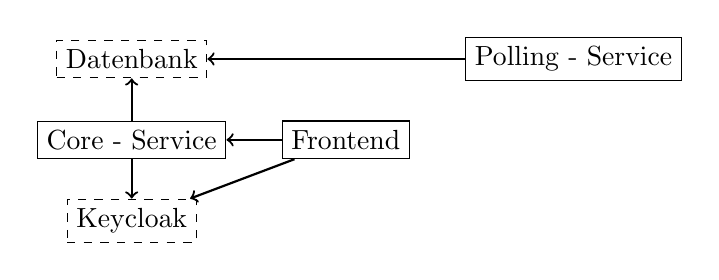
\begin{tikzpicture}
        \matrix [column sep=7mm, row sep=5mm] {
            \node (database) [draw, shape=rectangle, dashed] {Datenbank}; &&
            \node (polling_service) [draw, shape=rectangle] {Polling - Service}; \\
            \node (core_service) [draw, shape=rectangle] {Core - Service}; &
            \node (frontend) [draw, shape=rectangle] {Frontend}; \\
            \node (keycloak) [draw, shape=rectangle, dashed] {Keycloak}; \\
            };
            \draw[->, thick] (core_service) -- (database);
            \draw[->, thick] (frontend) -- (core_service);
            \draw[->, thick] (polling_service) -- (database);
            \draw[->, thick] (core_service) -- (keycloak);
            \draw[->, thick] (frontend) -- (keycloak);
        \end{tikzpicture}        
\caption{Diagramm – Darstellung der Service Architektur}
\end{figure}

\subsection{CI/CD Infrastrukture}
Um Code Qualität zu gewährleisten, wurde eine \ac{CI/CD} Infrastruktur entwickelt.
Diese ermöglicht es uns automatisiert Tests wie Unit und Integration Tests auszuführen und nach jeder Änderung aktuelle Versionen der Software zu veröffentlichen.
Da zum Beispiel eine neue veröffentlichung bei Änderungen auf der Master Branch stattfinden sollen, gibt es drei verschieden \ac{CI/CD} Pipelines.
Eine die nur Unit-Tests ausführt, eine die komplexe Tests ausführt und eine die eine neue Version veröffentlicht.

\subsubsection{Übersicht der Standard \ac{CI}-Pipline}
Die Standard \ac{CI}-Pipeline wird bei jedem Commit der nicht auf dem Master Branch stattfindet ausgeführt. Dabei hat die Standard Pipeline den geringsten Umfang and Aufgaben.
Diese führt nur die Unit-Tests aus, dazu muss der Code gecloned und alle Dependencies installiert werden. Somit sind direkt Fehler schon früh erkennbar, wenn diese Pipeline fehlschlägt.
\begin{figure}[!htbp]
    \centering    
    \usetikzlibrary{positioning}
    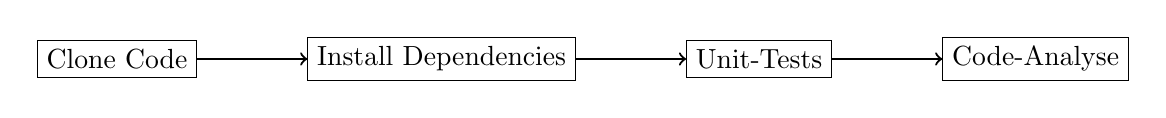
\begin{tikzpicture}
        \matrix [column sep=7mm, row sep=5mm] {
            \node (clone) [draw, shape=rectangle] {Clone Code}; &&
            \node (npm_setup) [draw, shape=rectangle] {Install Dependencies}; &&
            \node (unit_test) [draw, shape=rectangle] {Unit-Tests}; &&
            \node (sonar) [draw, shape=rectangle] {Code-Analyse}; \\
            };
            \draw[->, thick] (clone) -- (npm_setup);
            \draw[->, thick] (npm_setup) -- (unit_test);
            \draw[->, thick] (unit_test) -- (sonar);
        \end{tikzpicture}        
\caption{Diagramm – Darstellung der Standard \ac{CI}-Pipeline}
\end{figure}

\subsubsection{Übersicht der Pull-Request \ac{CI}-Pipline}
Die Pull-Request \ac{CI}-Pipeline wird ausgeführt sobald ein Pull-Request erstellt wird. Ihr Ziel ist es den jeweiligen Reviewer zu unterstützen, indem sie Tests und Code-Analyse durchführt.
Die Ergebnisse der Code Analyse werden direkt auf der Pull-Request Seite dargestellt. Sollten diese nicht den mindestanforderungen entsprechen, wird der Pull-Request dadurch blockiert.
Die Pipeline beinhaltet die selben Schritte wie die Standard Pipeline, sie erweitert diese lediglich um Integration-Tests.
\begin{figure}[!htbp]
    \centering    
    \usetikzlibrary{positioning}
    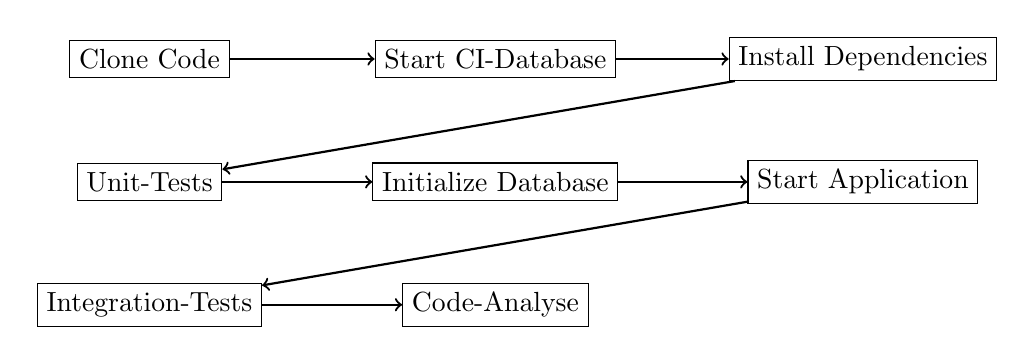
\begin{tikzpicture}
        \matrix [column sep=7mm, row sep=10mm] {
            \node (clone) [draw, shape=rectangle] {Clone Code}; &&
            \node (database) [draw, shape=rectangle] {Start \ac{CI}-Database}; &&
            \node (npm_setup) [draw, shape=rectangle] {Install Dependencies}; \\
            \node (unit_test) [draw, shape=rectangle] {Unit-Tests}; &&
            \node (init_db) [draw, shape=rectangle] {Initialize Database}; &&
            \node (start_app) [draw, shape=rectangle] {Start Application}; \\
            \node (int_test) [draw, shape=rectangle] {Integration-Tests}; &&
            \node (sonar) [draw, shape=rectangle] {Code-Analyse}; \\
            };
            \draw[->, thick] (clone) -- (database);
            \draw[->, thick] (database) -- (npm_setup);
            \draw[->, thick] (npm_setup) -- (unit_test);
            \draw[->, thick] (unit_test) -- (init_db);
            \draw[->, thick] (init_db) -- (start_app);
            \draw[->, thick] (start_app) -- (int_test);
            \draw[->, thick] (int_test) -- (sonar);
        \end{tikzpicture}
\caption{Diagramm – Darstellung der Pull-Request \ac{CI}-Pipeline}
\end{figure}

\subsubsection{Übersicht der Master \ac{CI}-Pipline}
Die Master \ac{CI}-Pipeline wird bei einen Commit auf den Master Branch ausgeführt. Dabei hat die Pipeline die Aufgabe den neuen Code auszurollen und sommit live zu bringen.
Zur Sicherheit werden auch wieder die Unit-Tests ausgeführt, damit auch wirklich sichergestellt wird, dass der Code lauffähig ist. Anschließend wird ein neues Docker-Image gebaut
welches dann in der Docker-Registry gespeichert wird. Nach erfolgreichem bauen des Images, wird die neue Image-Version in das Kubernetes-Depyoment geschrieben. Denn ArgoCD~\parencite{web/argocd} unser \ac{CD} Tool
erkennt automatisch Änderungen an den Kubernetes-Deployments und übernimmt diese. Somit sind die Code Änderungen an der Software in wenigen Minuten live ausgerollt.
\begin{figure}[!htbp]
    \centering    
    \usetikzlibrary{positioning}
    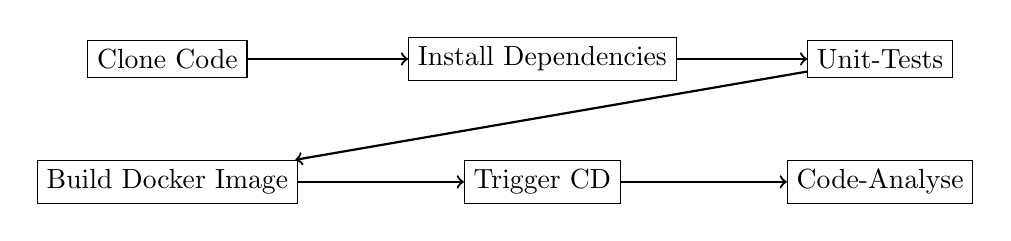
\begin{tikzpicture}
        \matrix [column sep=7mm, row sep=10mm] {
            \node (clone) [draw, shape=rectangle] {Clone Code}; &&
            \node (npm_setup) [draw, shape=rectangle] {Install Dependencies}; &&
            \node (unit_test) [draw, shape=rectangle] {Unit-Tests}; \\
            \node (docker_build) [draw, shape=rectangle] {Build Docker Image}; &&
            \node (trigger_cd) [draw, shape=rectangle] {Trigger \ac{CD}}; &&
            \node (sonar) [draw, shape=rectangle] {Code-Analyse}; \\
            };
            \draw[->, thick] (clone) -- (npm_setup);
            \draw[->, thick] (npm_setup) -- (unit_test);
            \draw[->, thick] (unit_test) -- (docker_build);
            \draw[->, thick] (docker_build) -- (trigger_cd);
            \draw[->, thick] (trigger_cd) -- (sonar);
        \end{tikzpicture}
\caption{Diagramm – Darstellung der Master \ac{CI}-Pipeline}
\end{figure}

\section{Mockups}

\section{Technische Änderungen zur anfänglichen Struktur} \label{tech_changes}
Im Laufe unseres Projektes sind einige technischen Hürden entstanden. Diese haben zum Teil dazu geführt das unsere ursprünglichen Requirements nicht mehr erfüllt werden konnten.
Deshalb wurden sie im Nachhinein dementsprechend leicht angepasst.

\begin{table}[h]
    \resizebox{\textwidth}{!}{\begin{tabular}{|p{8cm}|p{8cm}|}
    \hline
    Beschreibung der Änderung & Begründung der Änderung\\ \hline
    In der Plattform werden RSS Feeds keinen/wenig Inhalt anzeigen & Ein Großteil der im Internet vohandenen RSS Feeds verlinken nur auf Artikel und enthalten keinen Inhalt, was das Darstellen eines kompletten Artikels unmöglich macht. \\ 
    Das Hinzufügen von Feeds aus der Creator Page wurde zu einem Must-Have Requirement & Das anfänglich geplante manuelle Einbinden von Feeds ist als zu zeitaufwändig eingeschätzt worden. \\
    Die Creator Page wurde stark minimiert & Die geplanten Einstellungsmöglichkeiten der Creator Page wurden durch die Daten die ein RSS-Feeds liefert redundant. Um einen RSS-Feed hinzufügen ist lediglich die Adresse des Feeds notwendig. \\
    Die Funktionalität der Artikel Recommendations wurde minimiert & Dadurch das RSS Feeds heutzutage wenige bis keine Daten liefern, wurde beschlossen die Recommendations auf zufällig vorgeschlagene Artikel zu limitiert.  \\
    \hline
\end{tabular}}
\caption{Tabelle – Änderungen zur anfänglichen Struktur}
\end{table}

Die Creator Page wurde soweit in der Funktionalität gekürzt, dass nur noch die Adresse eines Feeds notwendig ist.
Jeder Nutzer kann Feeds hinzufügen, dass löschen eines Feeds können nur Administratoren. \\
Die Vorschläge für Artikel besteht durch die Anpassung nur noch aus einer zufälligen Auswahl von Artikeln.

